\subsection{BES1 Signalling Model} \label{bes1-model-section}

In this model and all subsequent models we aim to predict the behaviour of a single cell as it is pushed away from the quiescent centre (henceforth QC) by the growth and division of the cells beneath it. Within the meristematic zone, cells grow from a length of $4.5\um$ to $9\um$ over a period of approximately $18\h$ (\cite{verbelen2006}). However, cells may undergo one or more divisions during this time (\cite{goh2023}), so tracking the exact lineage of a single cell is difficult. For this reason, our model will only consider cells at $150\um$ or higher above the QC. 

\medskip

Prior to writing down a system of differential equations for our model, we need to rescale our data to be in terms of time instead of position. To do this, we map a position of $150\um$ above the QC to $t = 0\h$ and then use cell lineage data from \cite{goh2023} to determine a function that maps positions to times. The resulting position function is shown in Supplementary Figure \ref{sfig:position-function}.

\medskip

Our first model aims to predict the level of BR signalling within the cell as it moves away from the QC, measured in terms of the BES1 transcription factor. To do this, we will use a time-rescaled version of the BL concentration function shown in Supplementary Figures \ref{sfig:bl-bias} and \ref{sfig:bl-average} with $b = 0.5$ and $n = 50$. The model will be fit to time-rescaled fluorescence intensity data from the cell columns of a single \emph{A. thaliana} root (\cite{vukasinovic2021}). The BL concentration function and the data are shown in Supplementary Figure \ref{sfig:bes1-data}. It is important to note that there is likely additional plant-to-plant variance that remains unaccounted for due to the fact that the data comes from a single organism. 

\medskip

With our data prepared, we can now define an ODE model for the amount of BES1 transcript in terms of the BL concentration $B(t) = [\text{BL}]$. To do this, recall that Equation \eqref{bri1} gives us the concentration of bound BRI1 receptors $R_{B} = [\text{BRI1 BL}]$ in terms of $B(t)$, the dissociation constant $K_{d}$, and the total BRI1 concentration $R_{T} = [\text{BRI1}]$. For this model, we will fix $K_{d} = 10\nm$ (\cite{wang2001}) and $R_{T} = 62\nm$ (\cite{vanesse2012}) as in Figure \ref{fig:bri1-function}.

\begin{equation}
\label{rb}
R_{B}(B, R_{T}, K_{d}) = \frac{(B + R_{T} + K_{d}) - \sqrt{(B + R_{T} + K_{d})^{2} - 4 \cdot R_{T} \cdot B}}{2}
\end{equation}


When the concentration of bound BRI1 receptors $R_{B}$ is higher, the effects of the BIN2 signalling inhibitor are released, leading to increased production of BES1. Let $s_{\text{in}}$ denote the rate at which $R_{B}$ increases BES1 transcription. We also include a decay term with parameter $s_{\text{out}}$ to account for the degradation of the BES1 transcription factor over time. The intial condition is given by another parameter $\text{BES1}(0) = s_{0}$. Fitting this parameter will give us a non-dimensional estimate for the level of BES1 signalling at $150\um$ above the QC. 

\begin{equation}
\label{bes1}
\frac{d\text{BES1}}{dt} = s_{\text{in}}R_{B}(B, R_{T}, K_{d}) - s_{\text{out}}\text{BES1},\quad \text{BES1}(0) = s_{0}
\end{equation}

Since $R_{B}$ has $t$-dependence through the BL concentration function $B$, Equation \eqref{bes1} cannot be solved analytically and must be approximated using numerical methods. Before we show the results of these simulations, we present a visual summary of the model in Figure \ref{fig:bes1-model}.

\begin{figure}
    \centering
    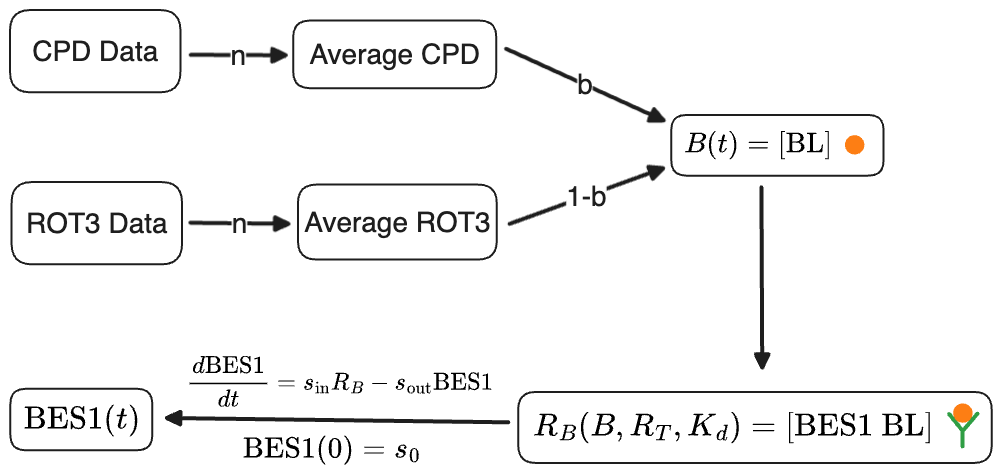
\includegraphics[width=13cm]{bes1-model.png}
    \caption{A visual depiction of the model up to this point. The extracellular BL concentration function $B(t)$ is computed using a moving biased average of the CPD and ROT3 biosynthetic enzymes. Then, $B(t)$ is used to determine the concentration of bound receptors $R_{B}$, building on the work of \cite{vanesse2012}. Finally, an ordinary differential equation model is used to express the BES1 transcription factor as a function of time through $R_{B}$.}
    \label{fig:bes1-model}
\end{figure}

\medskip

The BES1 function was approximated using a forward euler method with a time step of $0.01\h$. We evaluated the model using the Root-Mean-Squared Error (RMSE) metric. The formula is given in Equation \eqref{rmse} where $N$ denotes the number of observations. Each $y_{i}$ ($1 \leq i \leq N$) represents an observed value while each $f(t_{i})$ denotes the model output at time $t_{i}$.

\begin{equation}
\label{rmse}
\text{RMSE} =  \sqrt{\frac{1}{N}\sum_{i = 1}^{N} (y_{i} - f(t_{i}))^{2}}
\end{equation}


Additionally, the Akaike Information Criterion (henceforth AIC) presented in \cite{akaike1974} was used to compare the model presented (henceforth referred to as the complete model) with a linear and exponential regression on the BES1 signalling data. The AIC compares the relative quality of statistical models by considering both the goodness of fit and the informational complexity of the model. 

\begin{equation}
\label{aic}
\Delta \text{AIC} = 2k + N \ln\left( \frac{1}{N} \sum_{i = 1}^{N} (y_{i} - f(t_{i}))^{2}  \right) 
\end{equation}

In the equation above, $k$ denote the number of parameters in the model and $N$ is the number of observations. Since the AIC is used to compare models its absolute value is irrelevant. Therefore, the $\Delta \text{AIC}$ values presented in the forthcoming plots may be rescaled by a fixed constant to improve readability. The \verb|scipy.optimize.minimize| function from the scientific computation package \href{https://scipy.org/}{scipy} was used to determine the values of $s_{0} \in [0, 0.5]$, $s_{\text{in}} \in [0, 0.5]$, and $s_{\text{out}} \in [0, 0.5]$ that yielded the lowest error. Searching a larger parameter space did not produce a better fit (not shown).  Figure \ref{fig:bes1-model-fit} compares the fitted model to the experimental data and Table \ref{bes1-model-parameters} presents the optimized parameters. 

\begin{figure}
    \centering
    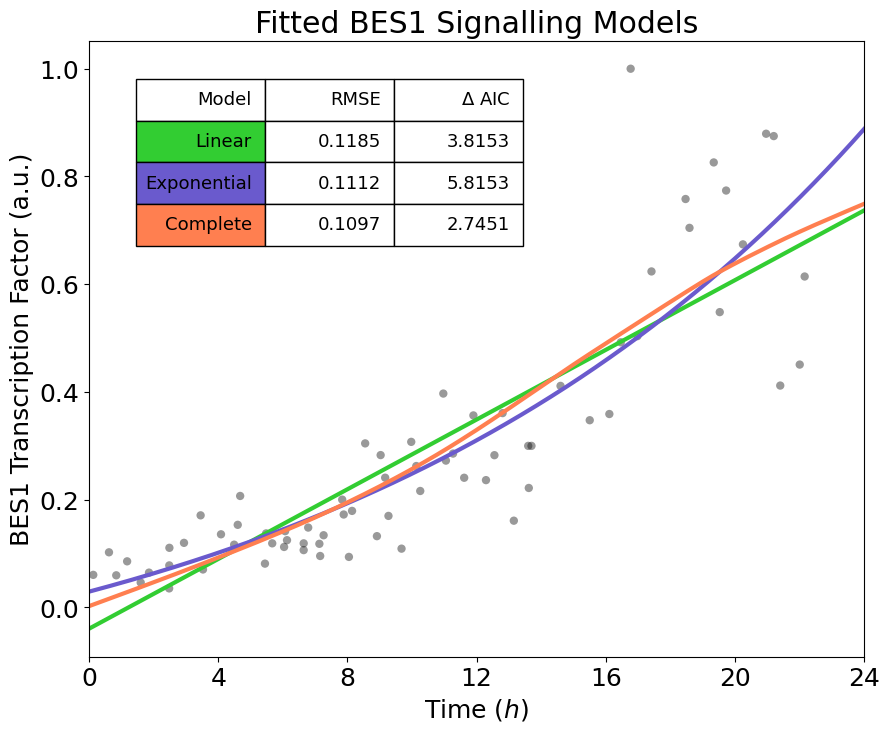
\includegraphics[width=13cm]{bes1-model-fit.png}
    \caption{Results of model fitting to the BES1 signalling data from \cite{vukasinovic2021}. The complete model was the best performing in terms of both absolute error and information-theoretic quality. } 
    \label{fig:bes1-model-fit}
\end{figure}

\medskip

\begin{center}
\label{bes1-model-parameters}
\begin{tabular}{ |c|c|c| } 
 \hline
 Parameter & Value & Units \\
 \hline
 $s_{0}$ & $2.35 \times 10^{-3}$ & $\text{BES1}$  \\
 $s_{\text{in}}$ & $4.79 \times 10^{-2}$ & $\text{BES1}/R_{B}\h$ \\ 
 $s_{\text{out}}$ & $3.53 \times 10^{-6}$ & $1/\h$ \\
 \hline
\end{tabular}
\end{center}

\medskip

The fitted parameter value $s_{\text{out}} = 3.53 \times 10^{-6}$ appears to be unreasonably low in the biological context of the problem. It suggests that BES1 has a half life of around $150$ days, which is unusually large. \cite{narsai2007} found that the the half life of transcription factors in \emph{A. thaliana} had a mean of $5.9\h$ and a median of $3.8\h$. However, some transcription factors had half lives above $24\h$. With these findings in mind, we can expect that the true value of $s_{\text{out}}$ is probably no more than $0.5$ and no less than $0.01$.

\medskip

To check if our model still performed reasonably well for values of $s_{\text{out}}$ within a biologically realistic range, we fixed $s_{0}$ to its fitted value and ran the model for a wide variety of possible $s_{\text{in}}$ and $s_{\text{out}}$ values. More precisely, we computed $100$ evenly spaced points from $s_{\text{in}} \in [0, 0.5]$ and $100$ evenly spaced points from $s_{\text{out}} \in [0, 0.5]$. This produced a lattice of $10\,000$ points in two-dimensional parameter space which were used to evaluate the model. Then, we ran the model at each of these points and plotted in the errors in Figure \ref{fig:bes1-model-heatmap}.

\begin{figure}
    \centering
    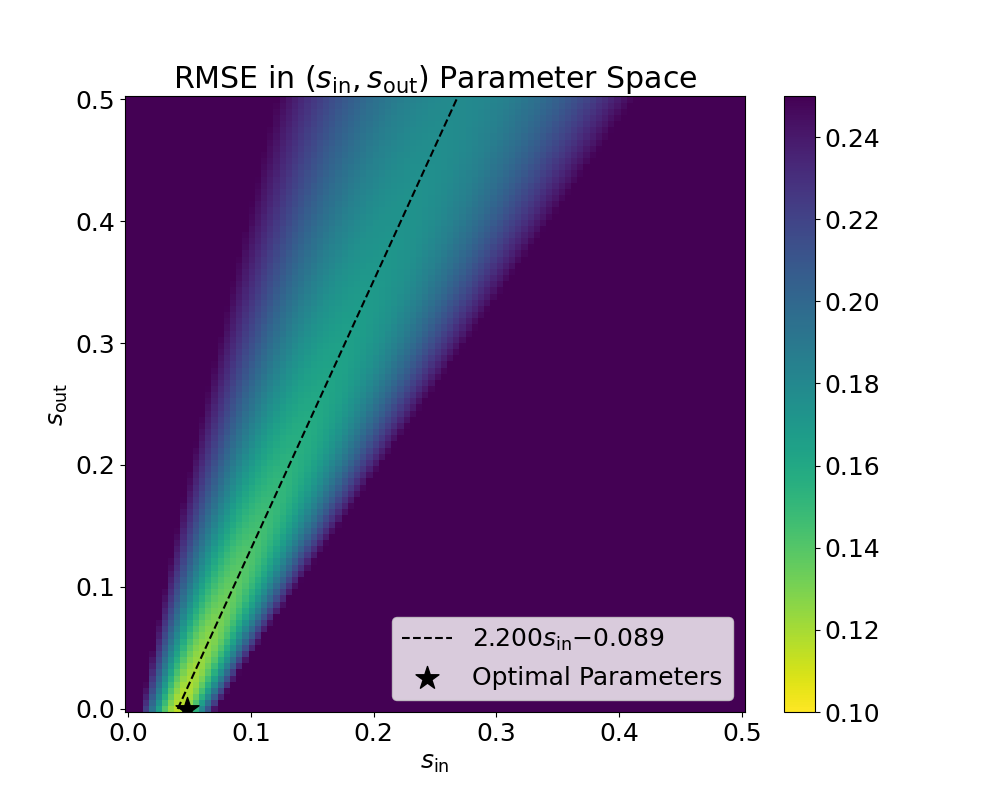
\includegraphics[width=13cm]{bes1-model-heatmap.png}
    \caption{Heatmap showing the model RMSE for a $100 \times 100$ grid of $(s_{\text{in}}, s_{\text{out}})$ parameter values. The initial condition $s_{0}$ was fixed to its fitted value of $2.35 \times 10^{-3}$. Regions of the plot shaded dark purple were truncated to an RMSE of $0.25$ and thus the actual RMSE at these points may be higher. The results of this process indicate a clear linear relationship between $s_{\text{in}}$ and $s_{\text{out}}$ which is given approximately by the linear function function $s_{\text{out}} = L(s_{\text{in}}) = 2.200s_{\text{in}} - 0.089$. }
    \label{fig:bes1-model-heatmap}
\end{figure}

\medskip

While the fitted parameter value $s_{\text{out}} = 3.53 \times 10^{-6}$ is probably not the true half life of the BES1 transcription factor as discussed previously, the parameter space search shows that the model also performs reasonably well for values of $s_{\text{out}}$ between $0.01$ and $0.5$. Lower values of $s_{\text{out}}$, which correspond with a longer BES1 half-life, produce slightly less error than higher values. This is indicated by the brighter yellow colour near the bottom of the dotted black line in Figure \ref{fig:bes1-model-heatmap}. In the regime where $s_{\text{out}}$ is small Equation \eqref{bes1} can be approximated as follows:


\begin{equation}
\label{bes1-sout-small}
\frac{\text{BES1}}{dt} = s_{\text{in}}R_{B} - s_{\text{out}}\text{BES1} \approx s_{\text{in}}R_{B} \Rightarrow \text{BES1} \approx s_{\text{in}} \int R_{B} \, dt
\end{equation}

This approximation indicates that the BES1 transcription factor accumulates over time in the cell and does not reach the maximum steady state value imposed by $s_{\text{out}}$. All of the biologically reasonable values for $s_{\text{out}}$ fall under this regime. For the sake of comparison, let us also consider the region of our parameter space where $s_{\text{out}}$ is large, which produces a less accurate fit. Under this regime we have the following approximation for the BES1 function:
$$
\text{BES1} = \frac{s_{\text{in}}R_{B}}{s_{\text{out}}} + \left( s_{0} - \frac{s_{\text{in}}R_{B}}{s_{\text{out}}} \right) e^{-s_{\text{out}}\text{BES1}} \approx \frac{s_{\text{in}}R_{B}}{s_{\text{out}}}
$$

When $s_{\text{out}}$ is large, the BES1 transcription factor rapidly reaches its steady state value, and is thus approximately proportional to $R_{B}$ over the domain. As mentioned previously, the actual system probably does not behaves this way since the model fits poorly to the data for larger values of $s_{\text{out}}$.

\medskip

The results of the parameter space search shown in Figure \ref{fig:bes1-model-heatmap} also indicate that if $s_{\text{in}}$ or $s_{\text{out}}$ can be determined through experiments, the other parameter value can also be estimated to a high degree of accuracy using the linear relationship $s_{\text{out}} = L(s_{\text{in}}) = 2.200s_{\text{in}} - 0.089$. This result is significant because it may be experimentally feasible to find $s_{\text{out}}$, the BES1 transcription factor decay constant, and use it to determine $s_{\text{in}}$, which would be difficult to determine experimentally. However, there are some caveats to this approach. Since the data has arbitrary units, quantifying $s_{\text{in}}$ would also require making exact measurements of the BES1 transcription factor and using them to rescale Equation \eqref{bes1} prior to using the linear relationship we identified. Additionally, there is some uncertainty in the behaviour of the BL concentration function $B(t)$ as the exact details of the BL biosynthetic pathway were left out of the model. That being said, the scale scale of the BL concentration ($\approx 1\nm$) is grounded in the literature (\cite{vanesse2012}). 
